\chapter{Planteamiento del problema}
%=============================================

%-----------------------------------
\section{Definición del problema}
%----------------------------------
En Colombia, el índice de robo de carros es cada vez mayor, segun datos de la Policía Nacional Colombiana, sólo el año 2019 los carros robados fueron 10.496, un promedio de 30 diarios (datos policia nacional colombiana). Bogotá encabeza el listado de ciudades donde más roban vehículos, seguido de Medellín, Cali, Bucaramanga y Barranquilla. Según cifras de la Policía, en Bogotá, durante el año 2018, habían sido denunciados 2.500 hurtos en parqueaderos. 
Segun un estudio realizado por Norza-Céspedes et \textit{al}, unas de las formas de controlar el hurto apunta a la prevención y disuasión \cite{PolNal}. En Colombia, un gran porcentaje de controles de entrada/salida de vehiculos son manuales y no ofrecen un sistema de registro de información que ayude a persuadir el hurto de vehiculos. 
Por otro lado, los establecimientos comerciales son cada vez más concurridos y el cliente muchas veces no encuentra sitio para parquear su automovil. Esto se debe en gran manera a que muchas personas dejan sus vehiculos en los parqueaderos de los centros comerciales, pero realmente no con el fin de realizar alguna compra; o si realizan una compra, permanecen por mucho tiempo después dentro del centro. Una solución para ello, es usar sistemas que controlen el tiempo de permanencia. En Colombia, muchos de estos controles de tiempo son manuales y además no ayudan a persuadir el hurto. Otros establecimientos utilizan software comerciales de empresas extranjeras que generalmente funcionan como una "caja negra" que cuando falla, el centro debe realizar el control manualmente ocasionando retrasos y congestionamiento. Además no permite la retroalimentación para corregir los errores. 
Una solución, tanto para disuadir el hurto de vehiculos como para descongestionar los parqueaderos, es implementar sistemas de inteligentes de visión artificial que aprovechen toda la tecnología actual y el avance de las ciencias de la computación. 
El problema de reconocimiento de placas de automoviles en Colombia plantea varios retos:
\begin{enumerate}
    \item Reconocer las placas de automoviles aun estando deterioradas, tal como lo muestra la figura \ref{fig:deteriorada}; 
     %--------------------
  \begin{figure}[H]
\begin{center}
   {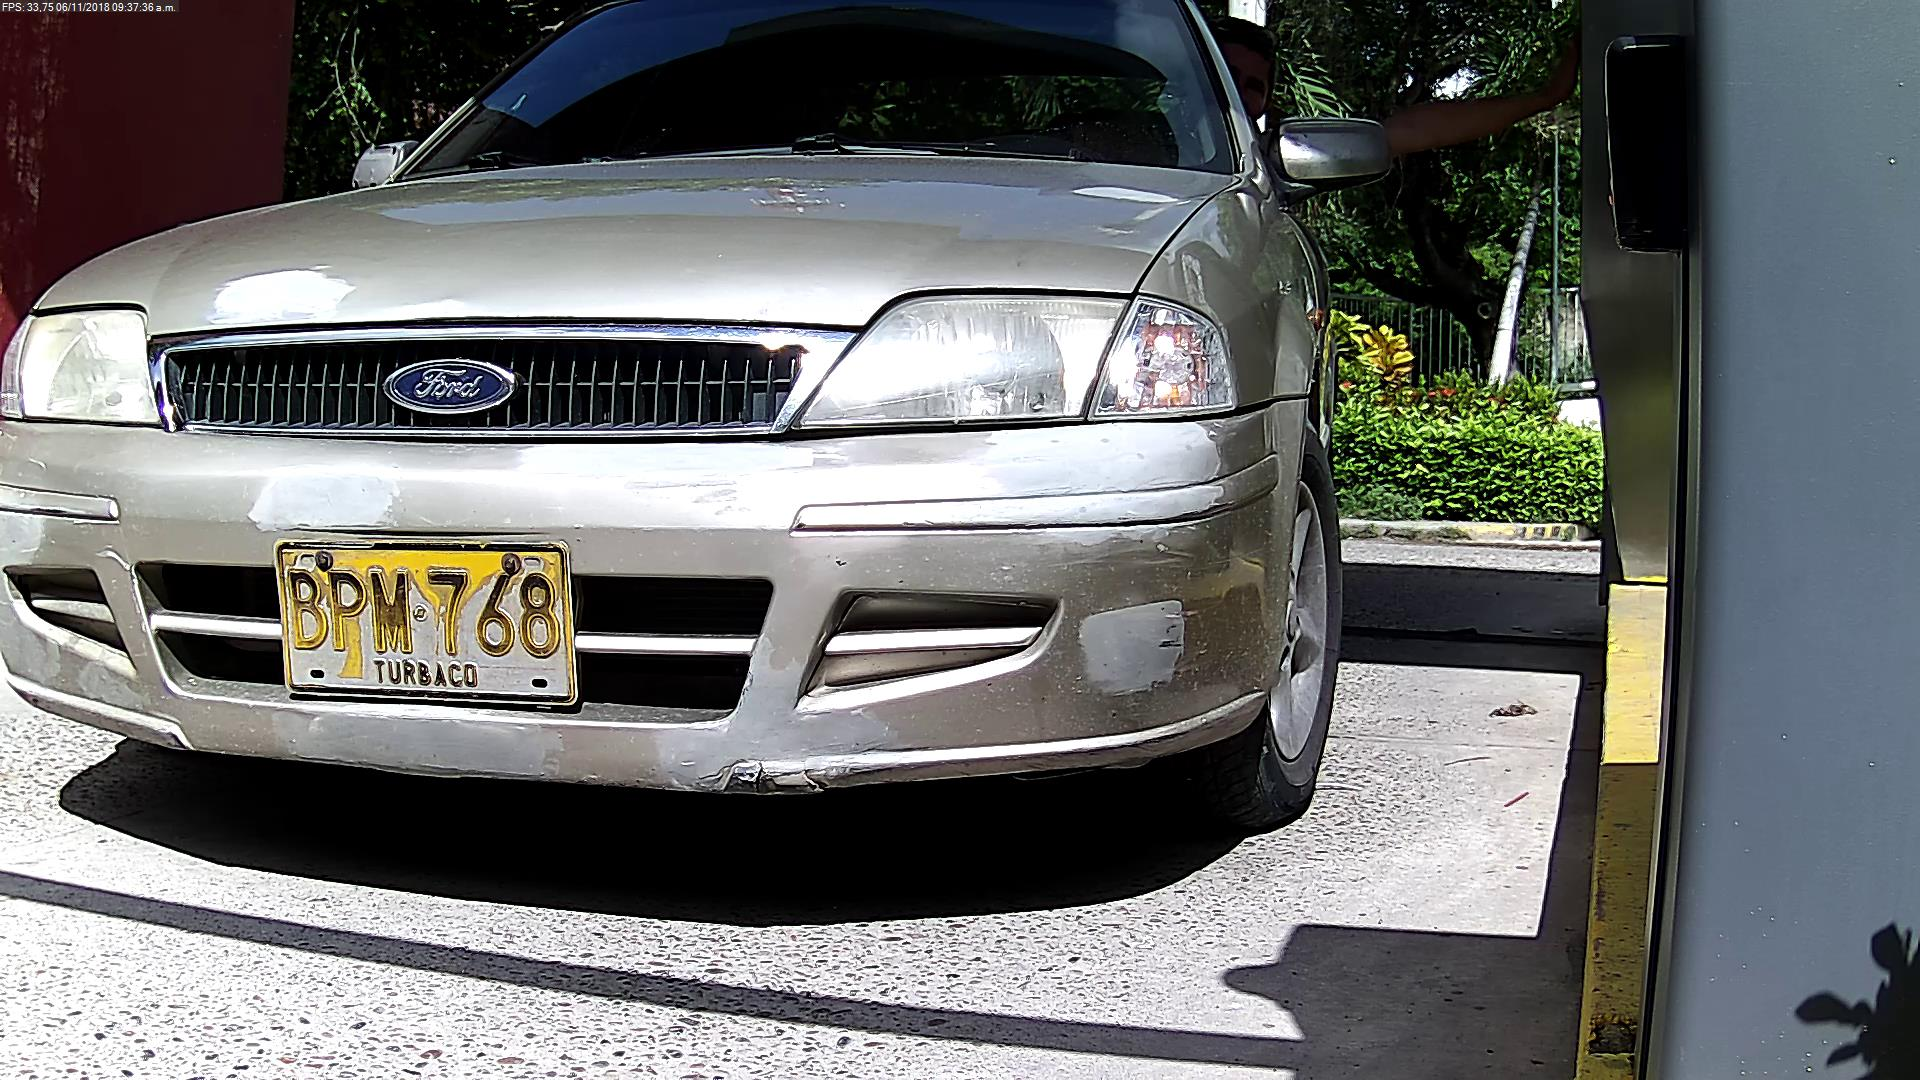
\includegraphics[width=0.8 \linewidth]{imagenes/Deterioradas/deteri.jpg}}
    \caption{Placa de automóvil con deterioro}
    \label{fig:deteriorada} 
\end{center}
\end{figure}
  %----------------------
\item Reconocer las placas de automoviles bajo condiciones ambientales adversas (iluminación, lluvia, etc), tal como lo muestra la figura \ref{fig:adversas}; 
    %--------------------
    \begin{figure}[H]
\begin{center}
   {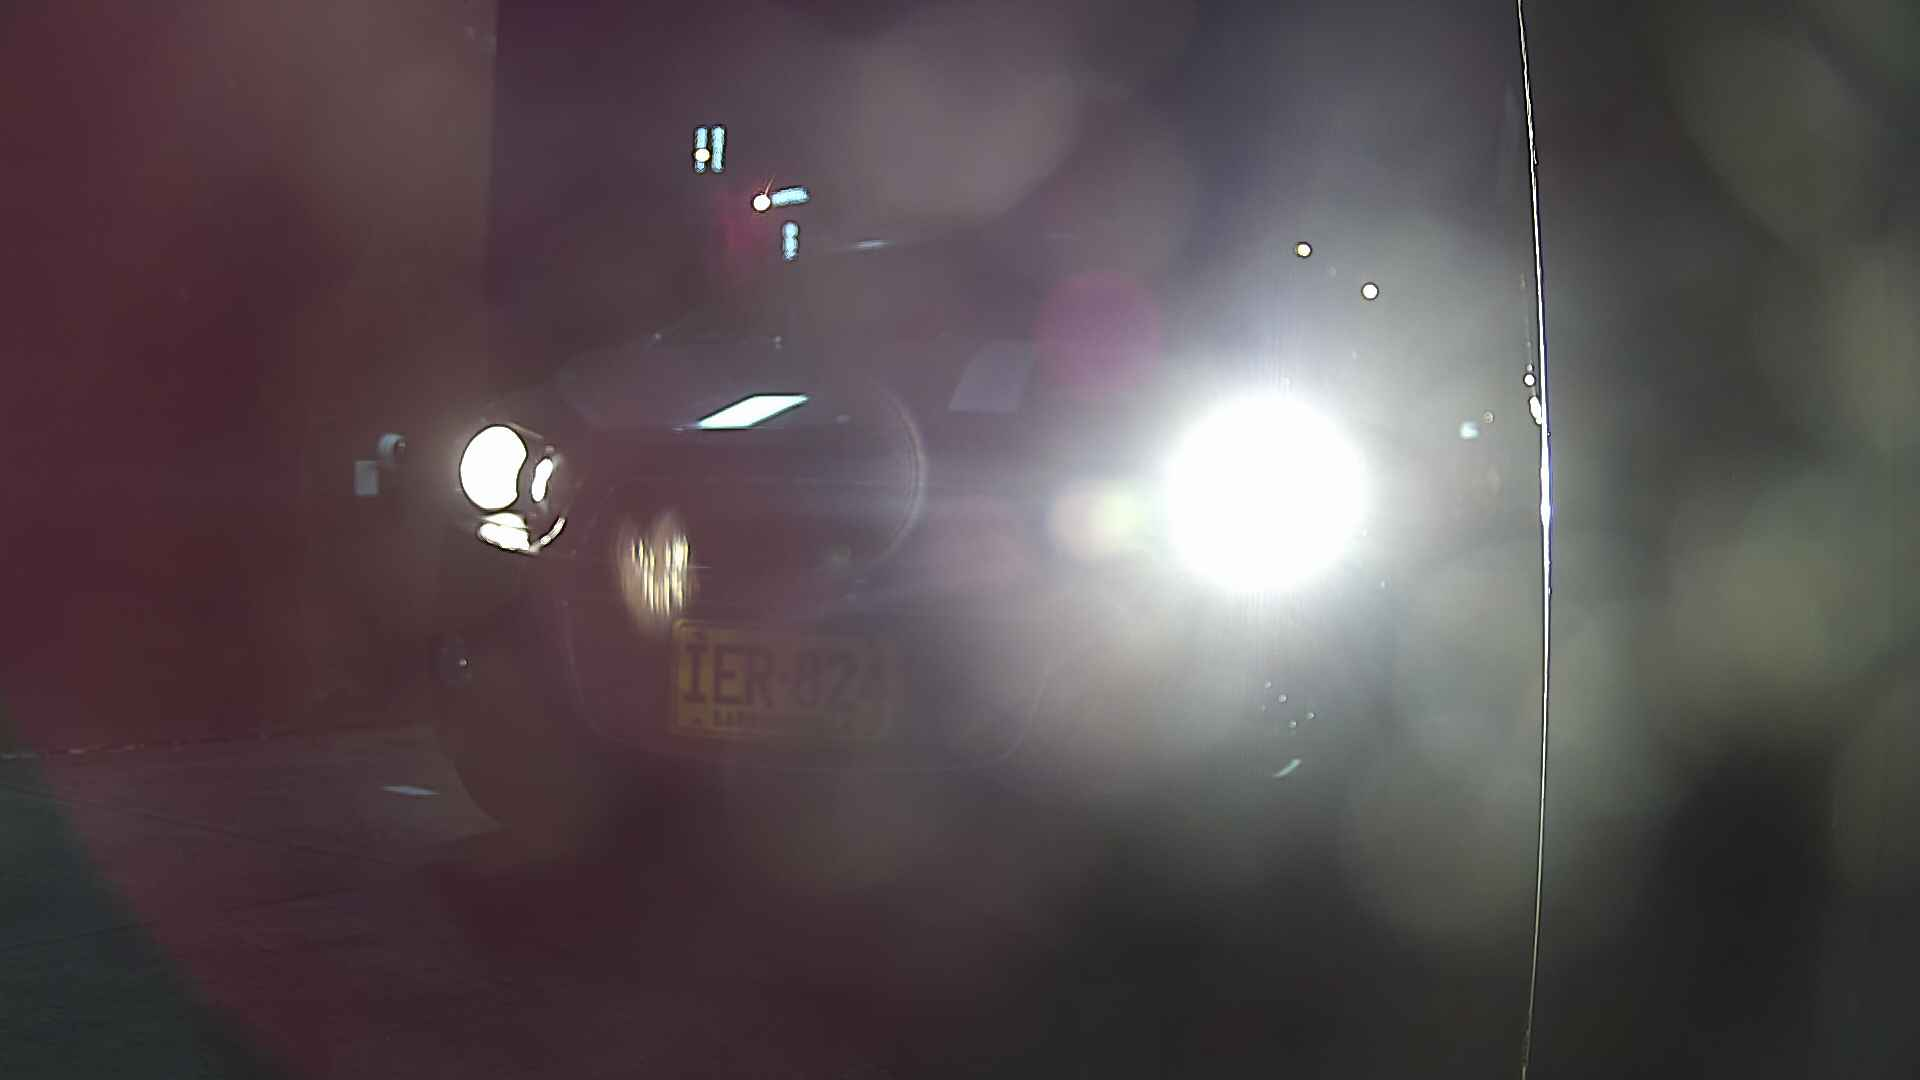
\includegraphics[width=0.8 \linewidth]{imagenes/Deterioradas/2018-11-04_17-57-36.jpg}}
    \caption{Placa de automóvil con condiciones adversas de iluminación}
    \label{fig:adversas} 
\end{center}
\end{figure}  
%-------------------------------
\item Reconocer las placas en diferentes perspectivas y escalamiento; 
    %--------------------------
    \begin{figure}[H]
\begin{center}
      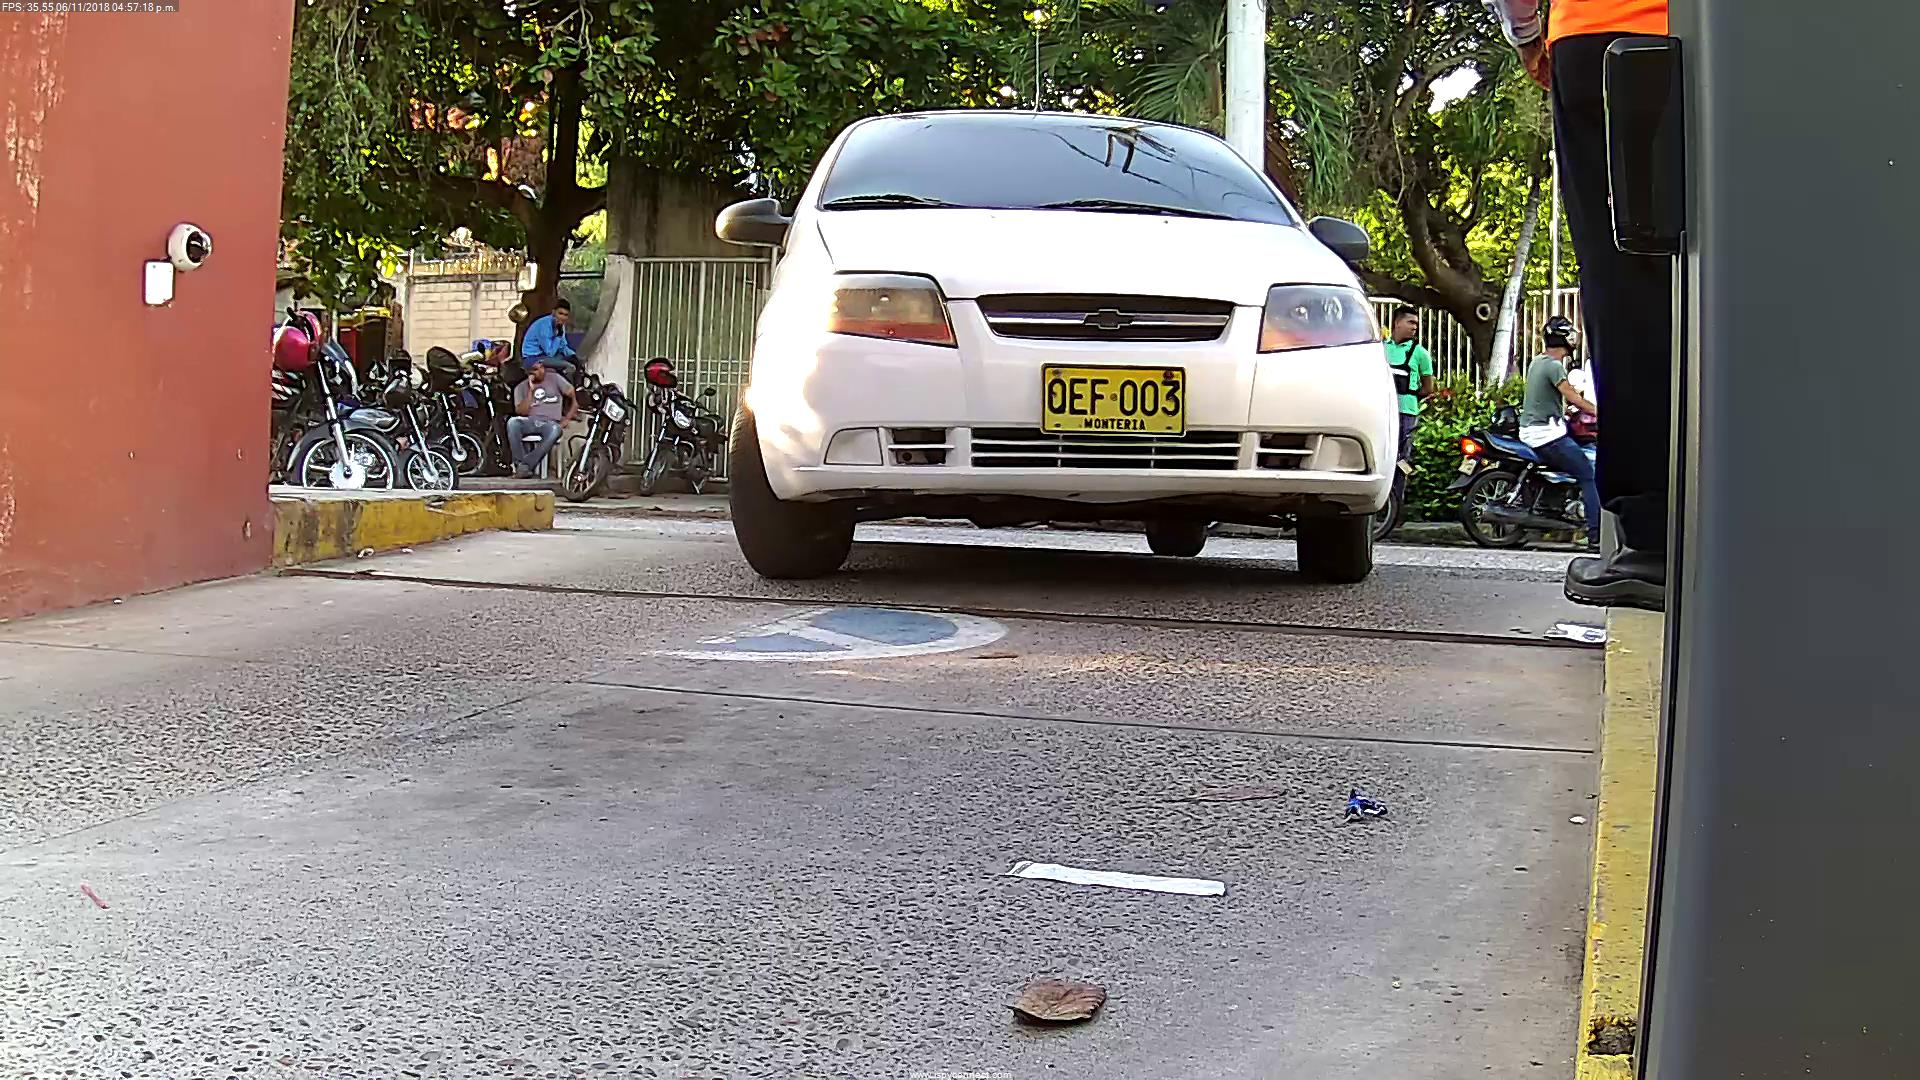
\includegraphics[width=0.8 \linewidth]{imagenes/Deterioradas/lejos.jpg}\\
    \caption{Placas con perspectiva lejana}
    \label{fig:lejos}  
\end{center}
\end{figure}
    %-----------------------
    \item Discriminar caracteres diferentes, pero con forma similar, tal como lo muestra la figura \ref{fig:similar};
    \end{enumerate}
 %--------------------
\begin{figure}[H]
\begin{center}
      \subfigure[]{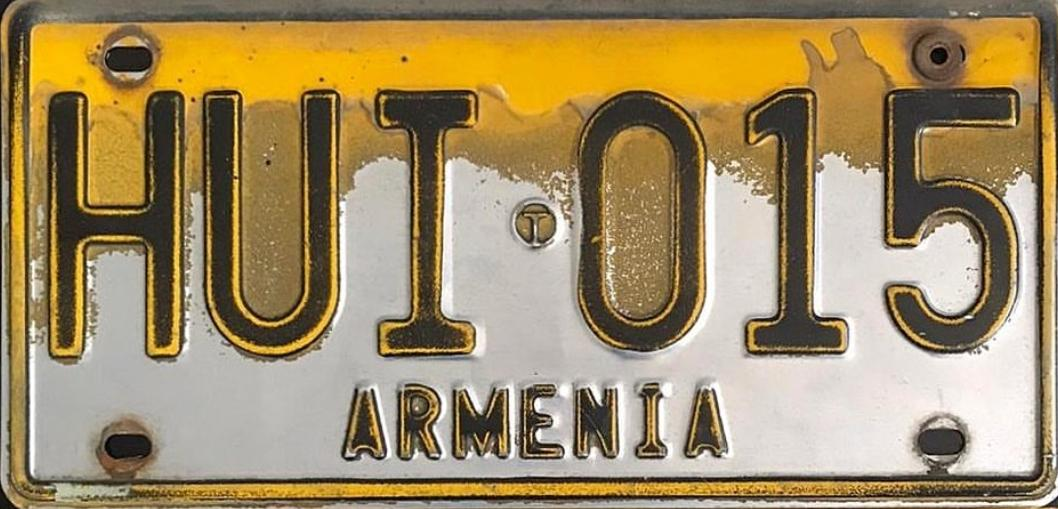
\includegraphics[width=0.4 \linewidth]{imagenes/Deterioradas/placa5.jpeg}}
    \subfigure[]{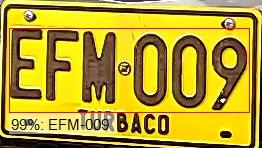
\includegraphics[width=0.35 \linewidth]{imagenes/Deterioradas/placa9.jpg}}
    \caption{Placas con caracteres similares: (a) letra I similar al número 1, (b) Letra E similar a la letra F}
    \label{fig:similar}  
\end{center}
\end{figure}
%------------------------------
   Para superar los retos planteados en el problema, nosotros proponemos usar Redes Neuronales Convolucionales, ya que son las ideales para el reconocimiento de objetos a partir de imágenes con demasiada variabilidad. Además, tales redes tienen incorporado una etapa de extracción de características que evitan su extracción manual que se realiza en el aprendizaje supervisado, para el posterior entrenamiento de una red neuronal convencional. El uso de RNC plantea unos retos técnicos, tales como: 
\begin{enumerate}
\item Conseguir una base de datos con placas colombianas debidamente etiquetada que permita el entrenamiento de la red; 
\item Escoger la mejor arquitectura de red que logre un excelente rendimiento.  
\end{enumerate}
%\newpage
\section{Pregunta de Investigación}

De acuerdo a los retos anteriormente planteados, la siguiente investigación trató de dar respuesta a las siguientes preguntas:

\begin{itemize}
    \item[i.] ¿Es posible mejorar el rendimiento de una RNC agregándole imágenes de caracteres de la base de datos chars74k a una base de datos de imágenes de caracteres segmentados de placas colombianas?
    \item[ii.]¿Qué tan experto es un sistema de reconocimiento de placas usando detección de objetos con redes neuronales mucho más rápidas, (Faster R-CNN)?
   
\end{itemize}

\section{Objetivo General}
Diseñar y elaborar un sistema experto para el reconocimiento de placas de automóviles en Colombia usando Redes Neuronales Convoluciones.
\section{Objetivos específicos}
\begin{itemize}
    \item Explorar y estudiar diferentes arquitecturas de RNC y las herramientas computacionales más usadas para su entrenamiento.

    \item Diseñar y construir una base de datos con imágenes de placas de automóviles en Colombia con alta variabilidad, para el entrenamiento y test de una  Red Neuronal Convolucional.

    \item Plantear una nueva arquitectura de RNC con alto rendimiento en el reconocimiento de placas de automoviles colombianas.
    
    \item Construir una base de datos con las coordenadas de caracteres de placas colombianas obtenidas usando Cuadros Delimitadores  (Bonding  Boxing) para entrenar una  Red  Neuronal  Convolucional mucho mas Ŕapida con propuesta de Regiones (Faster R-CNN). 
    
\end{itemize}
